\documentclass[acronym,symbols]{fei}
\usepackage[utf8]{inputenc}

\usepackage{subcaption} 
\usepackage{graphicx}
\usepackage{amsmath} % for the equation* environment
\usepackage{float}
\usepackage[portuguese]{algorithm2e}
\usepackage{biblatex}
\usepackage{listings}
\usepackage{chngcntr} 
\usepackage{appendix}
\usepackage{gensymb}
\counterwithout{footnote}{chapter}
\usepackage{siunitx}
\sisetup{output-exponent-marker=\ensuremath{\mathrm{e}}}
\renewcommand{\cftfigurepresnum}{Figura }
\setlength{\cftfigurenumwidth}{5.7em}
\usepackage{titling}

\title{Simulação e Otimização Estrutural - Atividade A1 }
\author{Felipe Estevão Coquito de Mello RA: 11.120.486-3\\ Vitoria Fedatto Stefaneli RA: 11.120.497-0}
\cidade{São Bernardo do Campo}
\instituicao{Centro Universitário FEI}

\addbibresource{Referencias.bib}
%\bibliographystyle{plain}
\bibliography{Referencias}
\graphicspath{ {Imagens/}, {Tabelas/}}

\begin{document}

\maketitle

\begin{folhaderosto}
 Relatório apresentado ao departamento de Engenharia Mecânica do Centro Universitário FEI, como parte dos requisitos de avaliação da disciplina MEP250 - Simulação e Otimização Estrutural. Solicitado pelo Prof. Dr. Marcelo Otávio.
\end{folhaderosto}

\listoffigures
\tableofcontents

\chapter{Introdução}

As simulações de análise estática são muito importantes quando se deseja conhecer o comportamento de objetos e materiais desde os mais simples até os mais complexos.
Portanto, o objetivo deste estudo é avaliar o comportamento de uma mola, através do \textit{Software} \textit{Ansys}, e verificar a necessidade de aplicação da não linearidade. 



\chapter{Hipóteses}

As hipóteses são as condições de contorno para a qual a nossa simulação serão contidas, e uma das mais importantes é entender se há ou não a necessidade de fazer uma analise não linear. Existem três formas de não linearidade, considerando o material, considerando que haverá contatos de corpos ou partes, e considerando altas deformações.

A primeira forma de não linearidade é a que envolve considerar o material de forma não linear, adicionando esse material usando o \textit{Engineering Data}, essa forma considera que o material sofrerá esforços que passe da região linear (zona elástica) da curva de tensão e deformação. Considerando que a função do material é ser uma mola, é esperado que ela trabalhe apenas na zona elástica, logo que apesar da deformação ela consiga voltar para o seu estado de origem.

A segunda forma, envolve o contato entre corpos ou partes, isso ocorre quando diferentes objetos ou partes do mesmo objeto começam a entrar em contato entre si podendo gerar tensões adicionais por essa interação, o nosso caso é uma mola logo é esperado que as espiras tenha interação entre si.

Por fim, temos a ultima que tem como função a analise do comportamento das deformações, para a analise se terá uma deformação acima do normal culminando na necessário da ativação do \textit{Large Deflection} o estudo preliminar é se a deformação for maior que 30\% do maior comprimento do objeto. Outra coisa interpresante de se observar é que o \textit{Large Deflection} não afeta no resultado caso não ocorra a alta deformação esperada, só aumenta o poder computacional necessária. Neste caso é esperado que ocorram altas deformações

As hipóteses que adotamos no final para o trabalho foram:
\begin{enumerate}
    \item Aluno 1 - Vitoria: 11.120.497-0 -> $F_x$ = - [60 + 2 x 0] -> $F_x$ = - 60 $N$
    \item Aluno 2 - Felipe: 11.120.486-3 -> $F_y$ = - [20 + 3 x 3] -> $F_y$ = - 29 $N$
    \item Aço Estrutural (ASME BPV)
    \item Material Linear
    \item Contacts ligados
    \item Large Deflctions ligado
\end{enumerate}

\chapter{Materiais}

O material é o começo de qualquer analise estrutural, neste caso o material definido na atividade foi o Aço Estrutural, já que estaremos trabalhando com uma mola é esperado que ela trabalhe no regime elástico, não é necessário procurar pelo Aço-estrutural não linear. O Aço Estrutural que o \textit{Ansys Workbench 2024 R1} é o tabelado pela \textit{ASME BPV Code from 1998, Section 8, DIv 2, Table 5-110.1}, Figura \ref{fig: tabela} com as propriedade definidas na Figura \ref{fig: propriedades}.

\begin{figure}[!htb]
    \centering
    \caption{Material selecionado}
    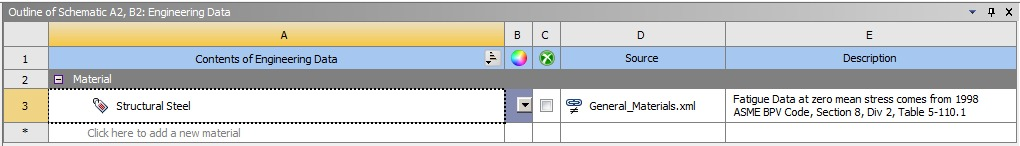
\includegraphics[width=0.8\linewidth]{Imagens/tabela ASME.jpeg}
    \smallcaption{Fonte: Autor}
    \label{fig: tabela}
\end{figure}

\begin{figure}[!htb]
    \centering
    \caption{Propriedades do material}
    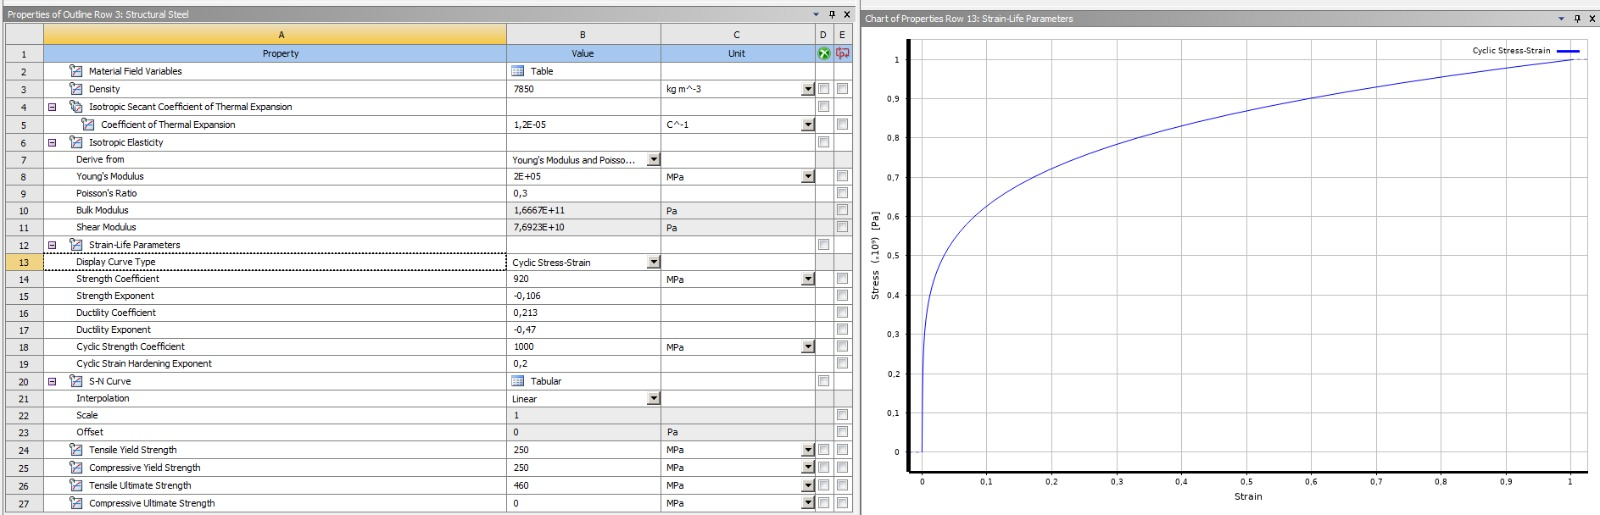
\includegraphics[width=0.8\linewidth]{Imagens/propriedades.jpeg}
    \smallcaption{Fonte: Autor}
    \label{fig: propriedades}
\end{figure}

Como é possível analisar na Tensão de escoamento, de 920 $MPa$ é abaixo da esperado para a construção de uma mola, sendo comumente feita de "Aço Mola com auto teor de carbono" ou "Aço Mola Inoxidável" \cite{centuryspring} e tendo como tensão de escoamento, entre de $R_{p0,2}$  de até 2800 $MPa$, segunda a fabricante \textcite{waelzholz} . Na analise preliminar é possível ver que as Tensões passam dos 920 $MPa$, Figura \ref{fig: preliminar}, chegando até 1029,2 $MPa$, o fato disso ocorrer é que o material não é o esperado para construção de uma Mola, como discutido anteriormente.

\begin{figure}[!htb]
    \centering
    \caption{Tensão Máxima prelimenear}
    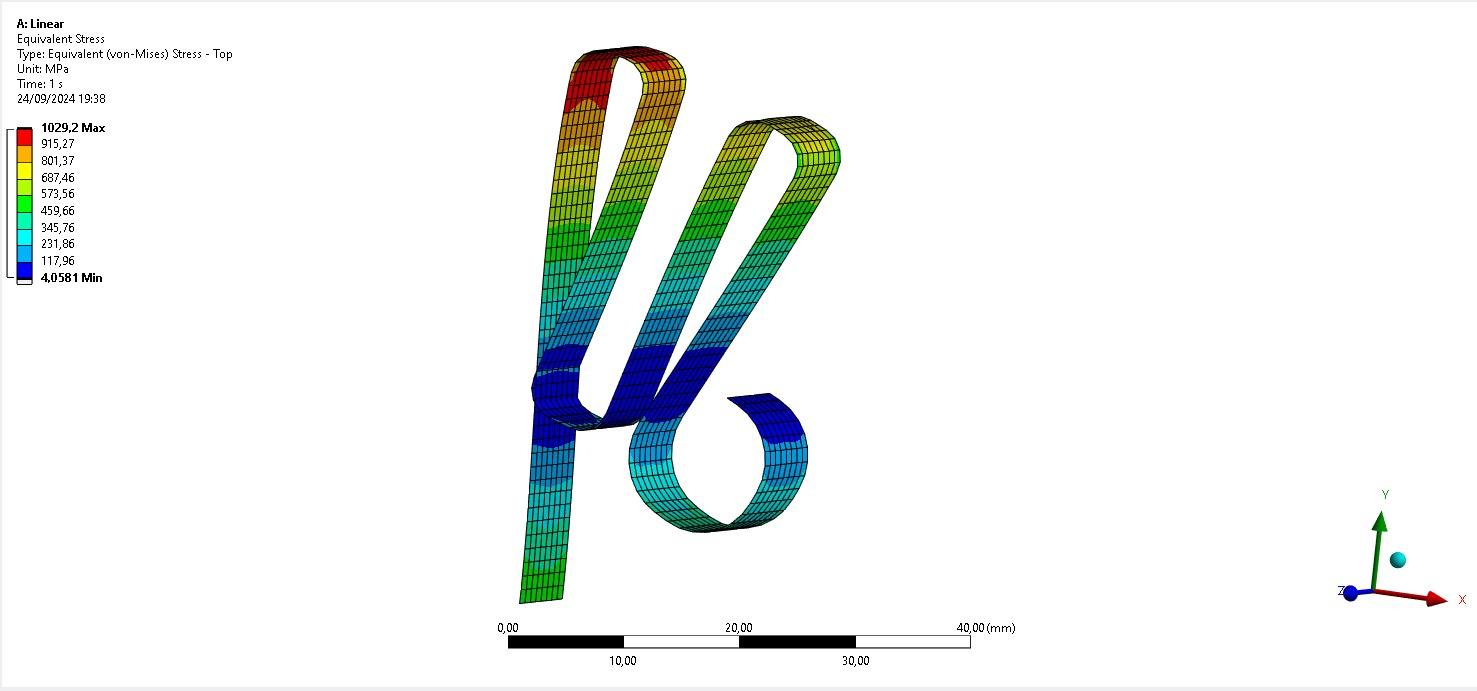
\includegraphics[width=0.8\linewidth]{Imagens/analise von-misses linear.jpeg}
    \smallcaption{Fonte: Autor}
    \label{fig: preliminar}
\end{figure}


\chapter{Geometria}

A geometria apresentada pelo professor é de uma mola de compressão. Tem em sua composição 4 espiras e espessura definida de 1 $mm$, é possível observar o objeto inteiro na Figura \ref{fig: geometria}. Por conta da sua baixa espessura a geometria é do tipo casca, onde a sua espessura tem dimensão desprezível em comparação as outras dimensões, como é possível observar na Figura \ref{fig: detalhes geometria}.

\begin{figure}[!htb]
    \centering
    \caption{Geometia da mola}
    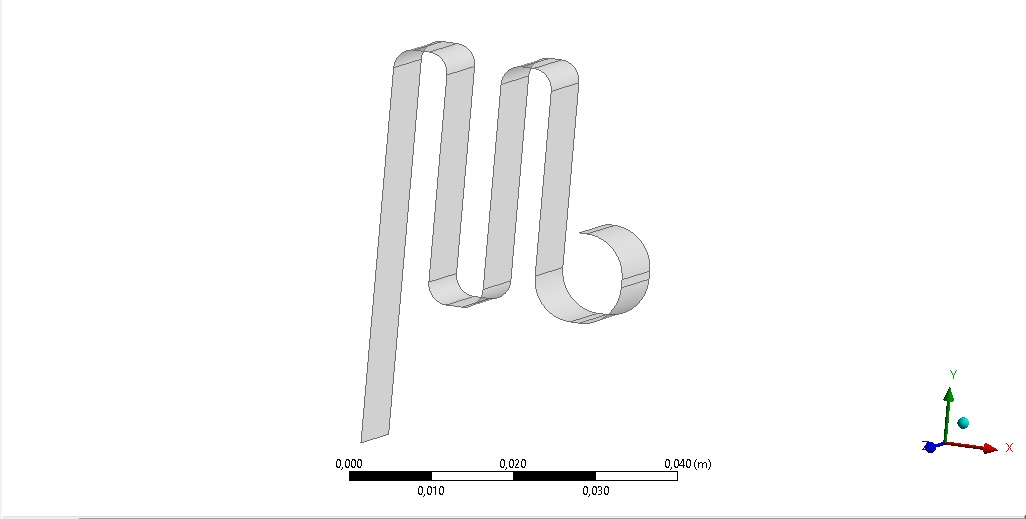
\includegraphics[width=0.9\linewidth]{Imagens/geometria.jpeg}
    \smallcaption{Fonte: Autor}
    \label{fig: geometria}
\end{figure}

\begin{figure}[!htb]
    \centering
    \caption{Configurações da geometia da mola}
    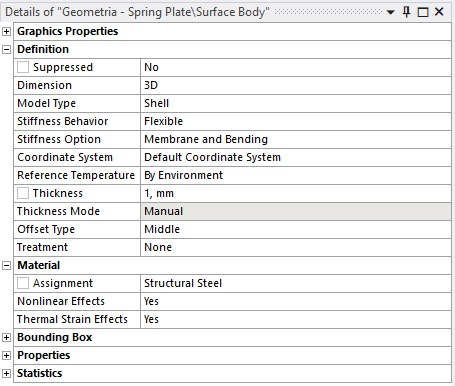
\includegraphics[width=0.5\linewidth]{Imagens/detalhes geometria.jpeg}
    \smallcaption{Fonte: Autor}
    \label{fig: detalhes geometria}
\end{figure}


\chapter{Modelo de Elementos Finitos (Malha)}

A malha é algo fundamental para a analise de elementos finitos, portanto a malha escolhida foi a quadrática com elementos de tamanho 1,2 $mm$. E foram obtidos 1394 elementos de malha. Todas as informações da malha estão mostradas na Figura \ref{fig: malha}.

\begin{figure}[!htb]
    \centering
    \caption{Características da malha}
    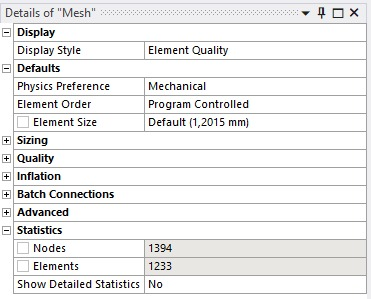
\includegraphics[width=0.5\linewidth]{Imagens/qualidade malha.jpeg}
    \smallcaption{Fonte: Autor}
    \label{fig: malha}
\end{figure}

Uma malha considerada boa para a simulação deve ter todos os elementos com qualidade acima de 0,25. Então é necessário verificar a qualidade da mesma. A malha, com as características descritas acima, teve, como pior resultado de qualidade 0,55638, portanto, não foi necessário fazer nenhuma alteração. As Figuras
\ref{fig: malha colorida} e \ref{fig: grafico malha colorida} mostram a malha e o gráfico da qualidade dos elementos de malha, respectivamente.

\begin{figure}[!htb]
    \centering
    \caption{Malha}
    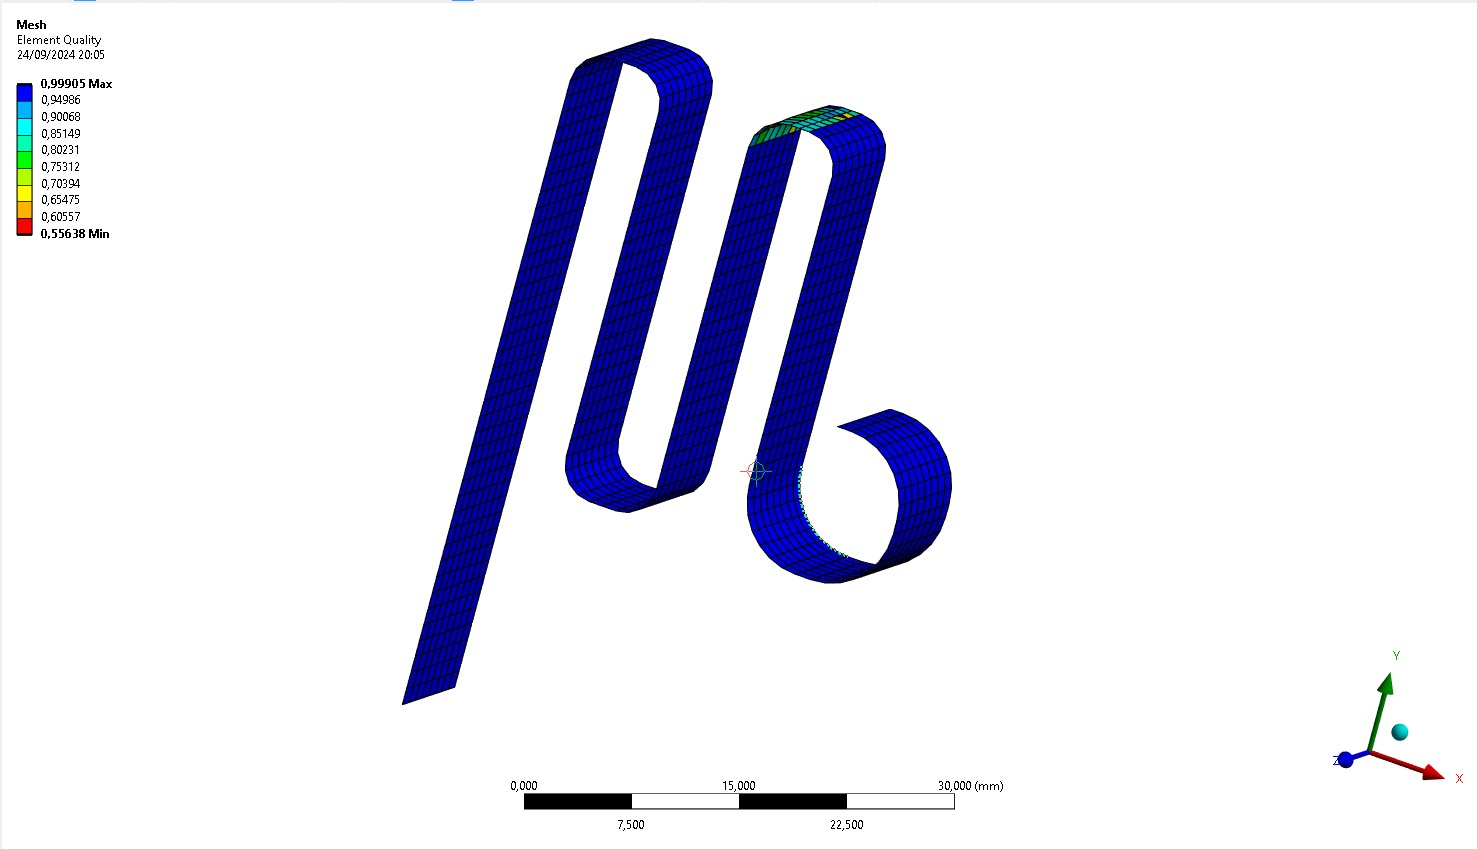
\includegraphics[width=0.7\linewidth]{Imagens/qualidade-malha.jpeg}
    \smallcaption{Fonte: Autor}
    \label{fig: malha colorida}
\end{figure}

\begin{figure}[!htb]
    \centering
    \caption{Gráfico de qualidade da malha}
    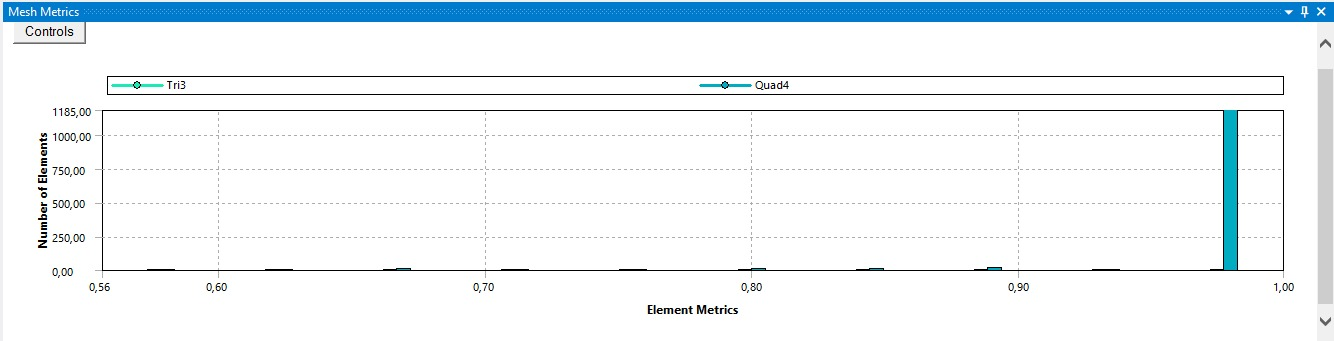
\includegraphics[width=0.7\linewidth]{Imagens/grafico qualid malha.jpeg}
    \smallcaption{Fonte: Autor}
    \label{fig: grafico malha colorida}
\end{figure}


\chapter{Apoios, Carregamentos e Contatos}

Os apoios, carregamentos e contatos, são a base para definir o que acontecerá com nosso objeto e segue as hipóteses abordadas anteriormente. Para a forma de contato foi escolhido um ponto de contato fixo na base do elemento, considerando assim que este ponto terá a maior força de reação pois está fixo ao 'chão' não tendo liberdade para movimentar-se, Figura \ref{fig: fixed suport}.

\begin{figure}[!htb]
    \centering
    \caption{Fixed suport}
    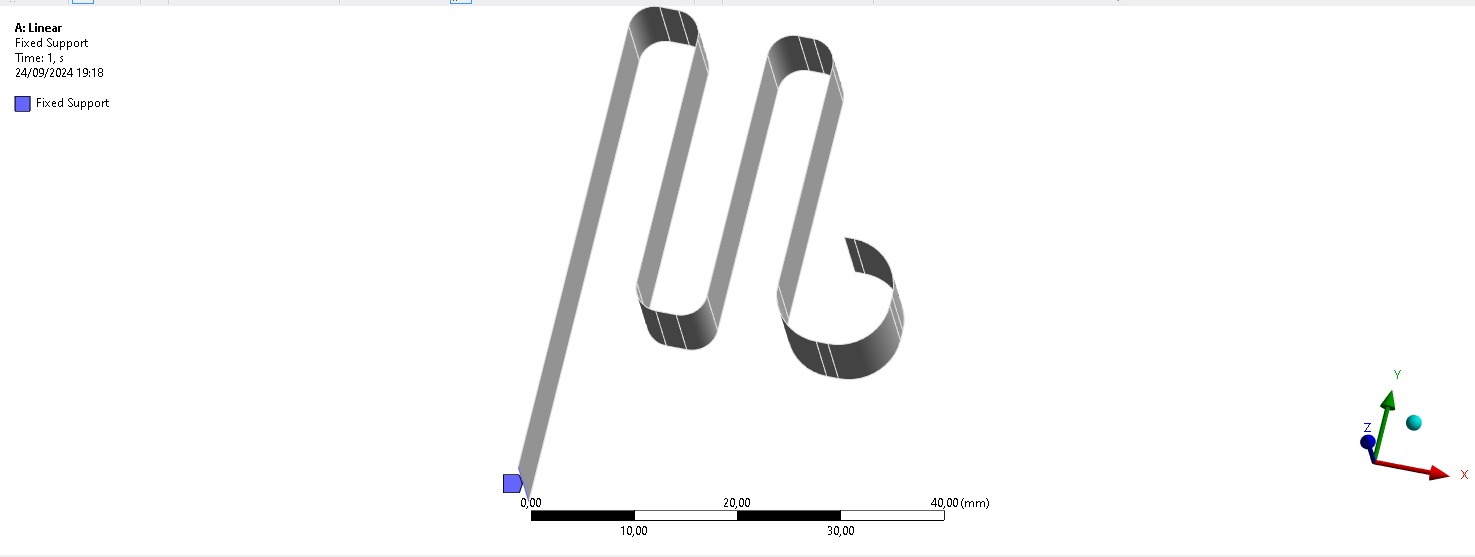
\includegraphics[width=1\linewidth]{Imagens/fixed suport.jpeg}
    \smallcaption{Fonte: Autor}
    \label{fig: fixed suport}
\end{figure}

Em seguida foi definido as forçar seguindo a formulação que o professor ofereceu sendo: $F_x$ = – [60 + 2 x (último algarismo do RA)aluno1] e $F_y$ = – [20 + 3 x (último algarismo do RA)aluno2], seguindo essa formula nossas forças foram:

\begin{itemize}
    \item Aluno 1 - Vitoria: 11.120.497-0 -> $F_x$ = - [60 + 2 x 0] -> $F_x$ = - 60 $N$
    \item Aluno 2 - Felipe: 11.120.486-3 -> $F_y$ = - [20 + 3 x 3] -> $F_y$ = - 29 $N$
\end{itemize}

Essas forças foram aplicadas a outra extremidade da mola como apresentado na Figura \ref{fig: força}.

\begin{figure}[!htb]
    \centering
    \caption{Força}
    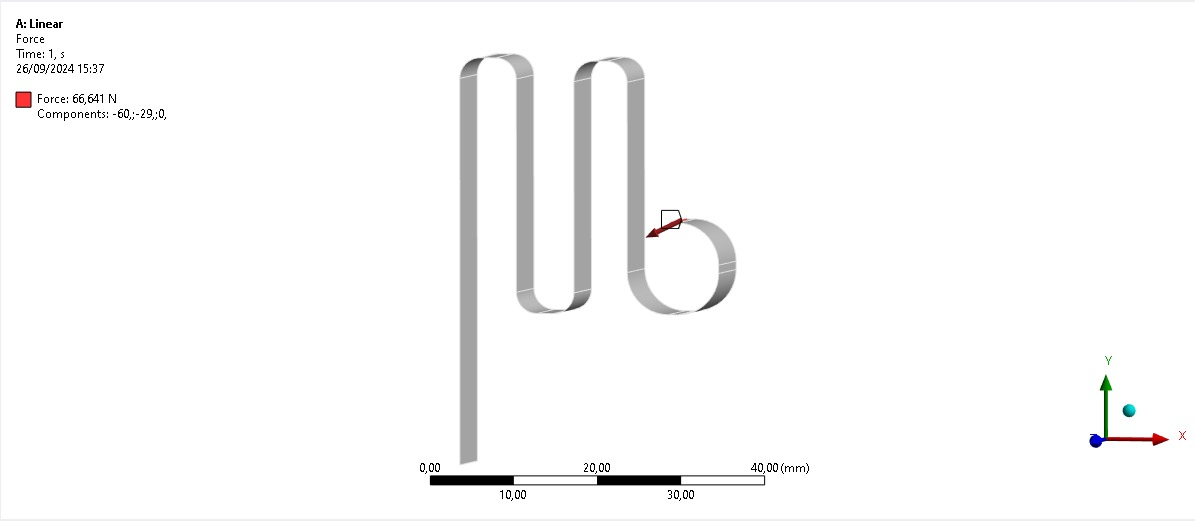
\includegraphics[width=1\linewidth]{Imagens/força.jpeg}
    \smallcaption{Fonte: Autor}
    \label{fig: força}
\end{figure}

Como elaborado nas hipóteses é esperado que as parte de duas espiras se toquem, logo é necessário a adição de possíveis pontos de contatos, que estabelecemos nos pontos azul e vermelho da Figura \ref{fig: contatos}. As propriedades desse contato foram definidas considerando ligado o \textit{Shell Thickness Effect} pois a espessura é miníma é como abas \textit{Shell Thickness Face} \textit{Top}, como obsedado na Figura \ref{fig: contato frictionless}.

\begin{figure}[!htb]
    \centering
    \caption{Contatos}
    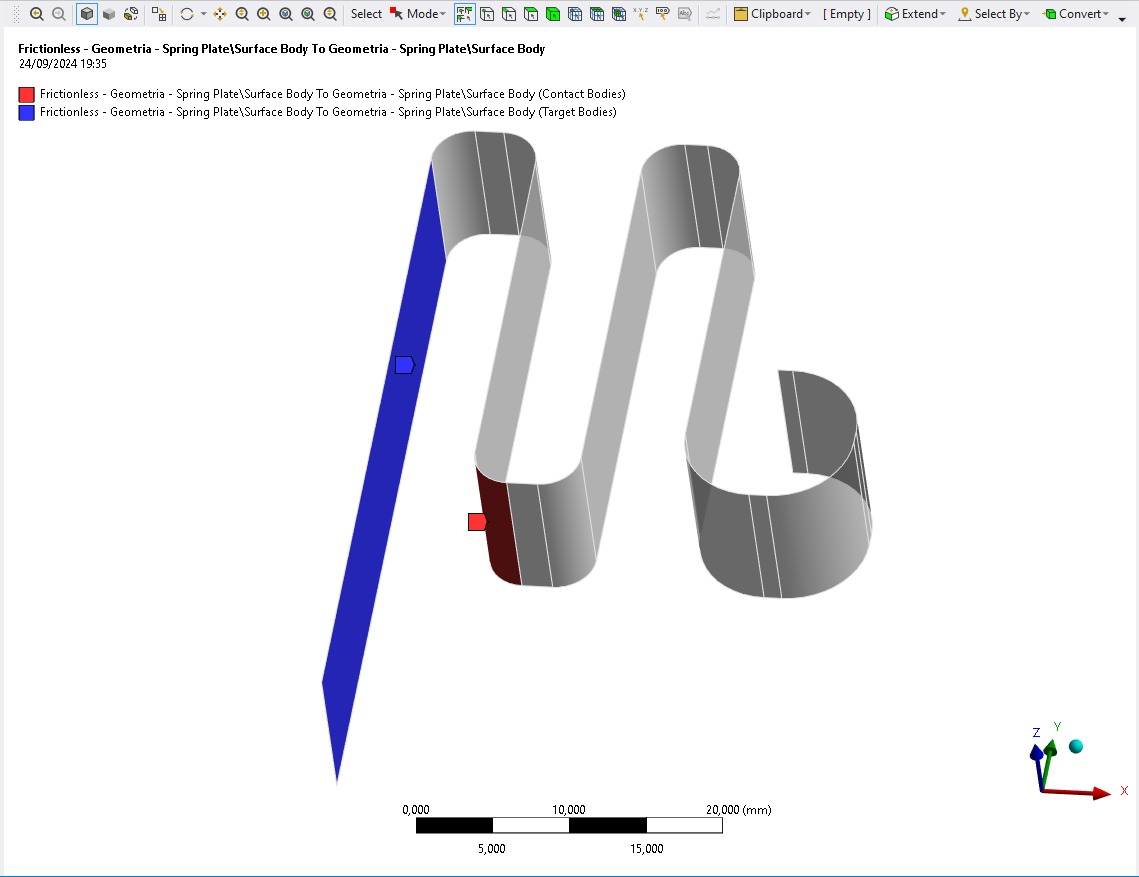
\includegraphics[width=0.8\linewidth]{Imagens/contatos.jpeg}
    \smallcaption{Fonte: Autor}
    \label{fig: contatos}
\end{figure}

\begin{figure}[!htb]
    \centering
    \caption{Contato frictionless}
    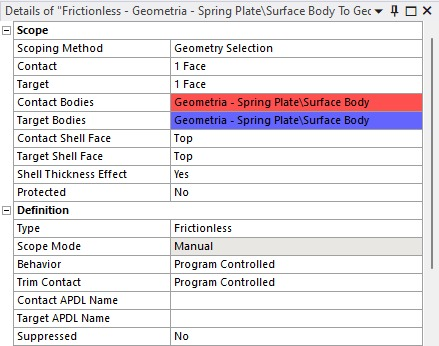
\includegraphics[width=0.6\linewidth]{Imagens/contato frictionless.jpeg}
    \smallcaption{Fonte: Autor}
    \label{fig: contato frictionless}
\end{figure}


\chapter{Resultados e Discussões}

Feitas as simulações iniciais com a geometria em comportamento linear, foi possível observar que houve uma deformação muito grande e, também, uma tensão equivalente muito maior que a tensão máxima que o material suporta. A Figura \ref{fig: deflinear} e a Figura \ref{fig: vonmisseslinear} mostram esses comportamentos.
\begin{figure}[!htb]
    \centering
    \caption{Deformação total linear}
    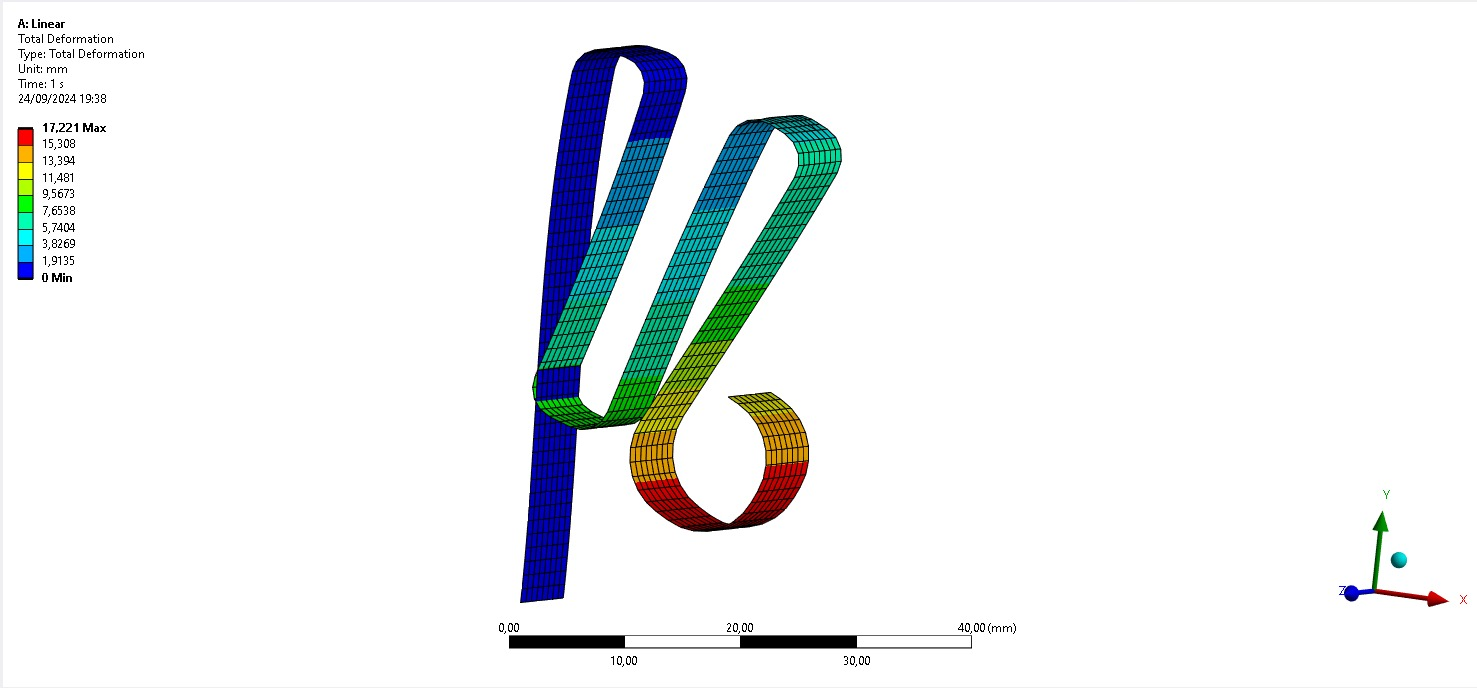
\includegraphics[width=0.7\linewidth]{Imagens/deformação total linear.jpeg}
    \smallcaption{Fonte: Autor}
    \label{fig: deflinear}
\end{figure}

\begin{figure}[!htb]
    \centering
    \caption{Tensão equivalente linear}
    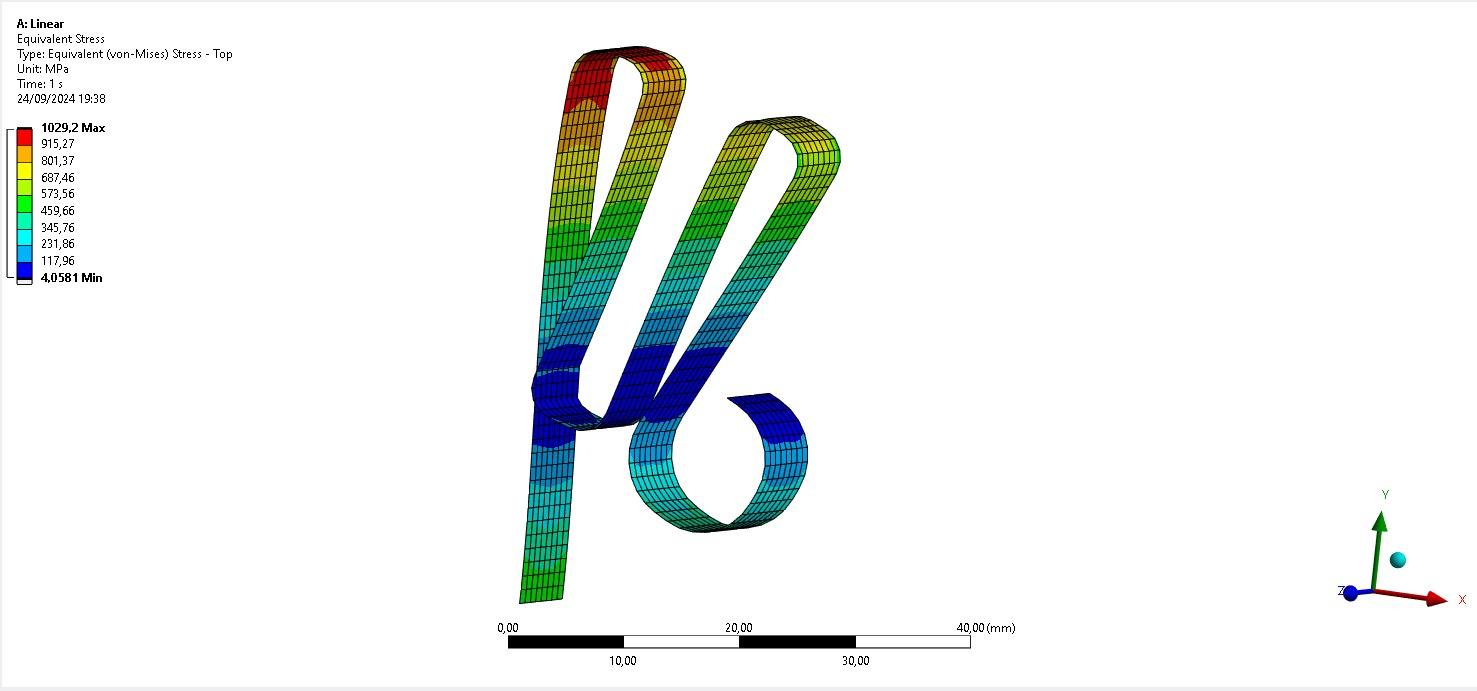
\includegraphics[width=0.7\linewidth]{Imagens/analise von-misses linear.jpeg}
    \smallcaption{Fonte: Autor}
    \label{fig: vonmisseslinear}
\end{figure}

Após aplicadas as condições de não-linearidade na mola (contato e large deflection), foi possível observar que para uma mesma força o deslocamento, em comparação com a simulação linear diminuiu significativamente, como é possível ver nas Figuras \ref{fig: fxd l} e \ref{fig: fxd nl}, que mostram os gráficos de força x deslocamento da comportamento linear e não-linear, respectivamente.
%Gráficos de convergência de força e de força vs. deslocamento.

%Explicar os resultados obtidos baseando-se nas hipóteses adotadas e na segurança do projeto em questão.


\begin{figure}[!htb]
    \centering
    \caption{Gráfico força x deslocamento linear}
    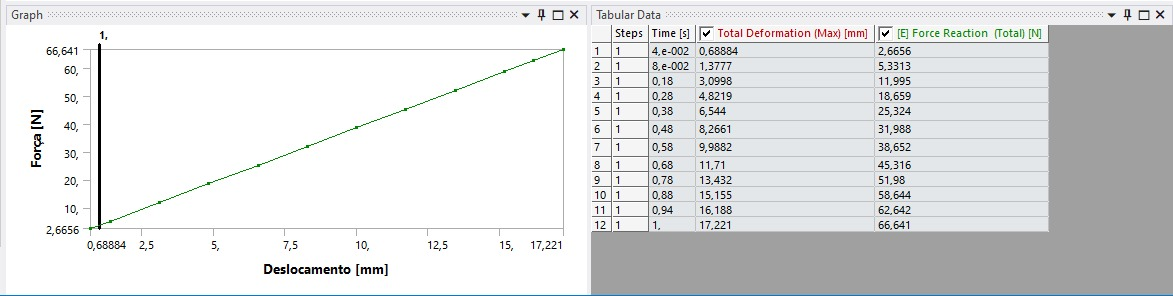
\includegraphics[width=0.6\linewidth]{Imagens/F x desloc linear.jpeg}
    \smallcaption{Fonte: Autor}
    \label{fig: fxd l}
\end{figure}

\begin{figure}[!htb]
    \centering
    \caption{Gráfico força x deslocamento não-linear}
    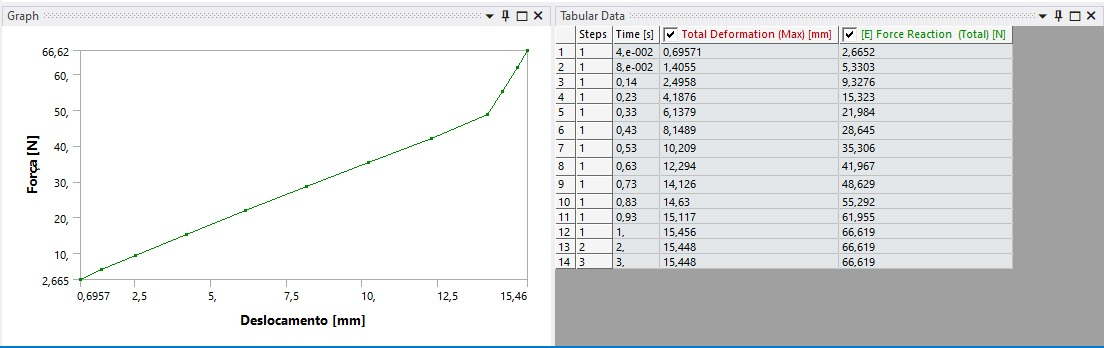
\includegraphics[width=0.6\linewidth]{Imagens/F x desloc nao linear.jpeg}
    \smallcaption{Fonte: Autor}
    \label{fig: fxd nl}
\end{figure}

Pode-se notar, também que a tensão equivalente de von-Misses diminuiu bastante, ficando, assim, abaixo do limite de tensão máxima do material. A Figura \ref{fig: vonmissesnl} mostra esse comportamento.

\begin{figure}[!htb]
    \centering
    \caption{Tensão equivalente não linear}
    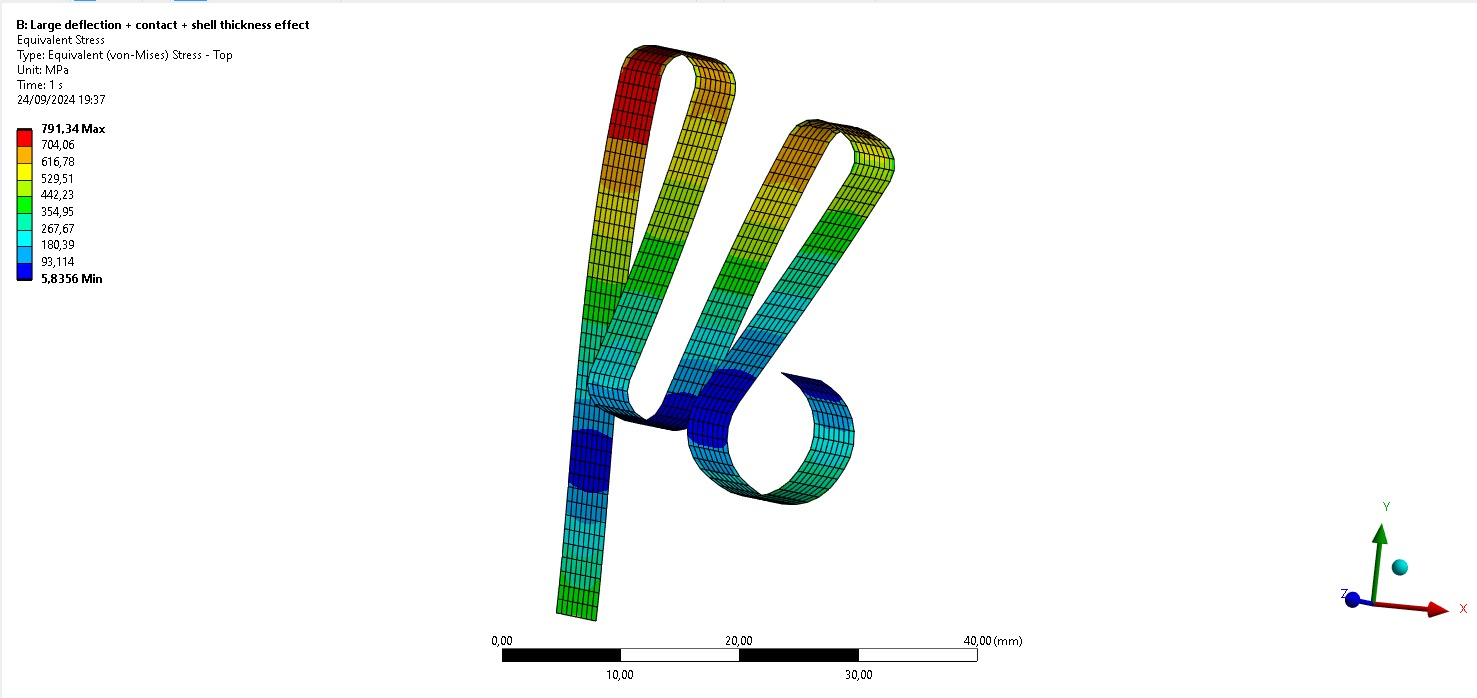
\includegraphics[width=0.7\linewidth]{Imagens/analise von misses nao linear.jpeg}
    \smallcaption{Fonte: Autor}
    \label{fig: vonmissesnl}
\end{figure}

Também foi possível observar que a deformação foi menor após a utilização do comportamento não linear, como mostra a Figura \ref{fig: defnl}.

\begin{figure}[!htb]
    \centering
    \caption{Deformação total não linear}
    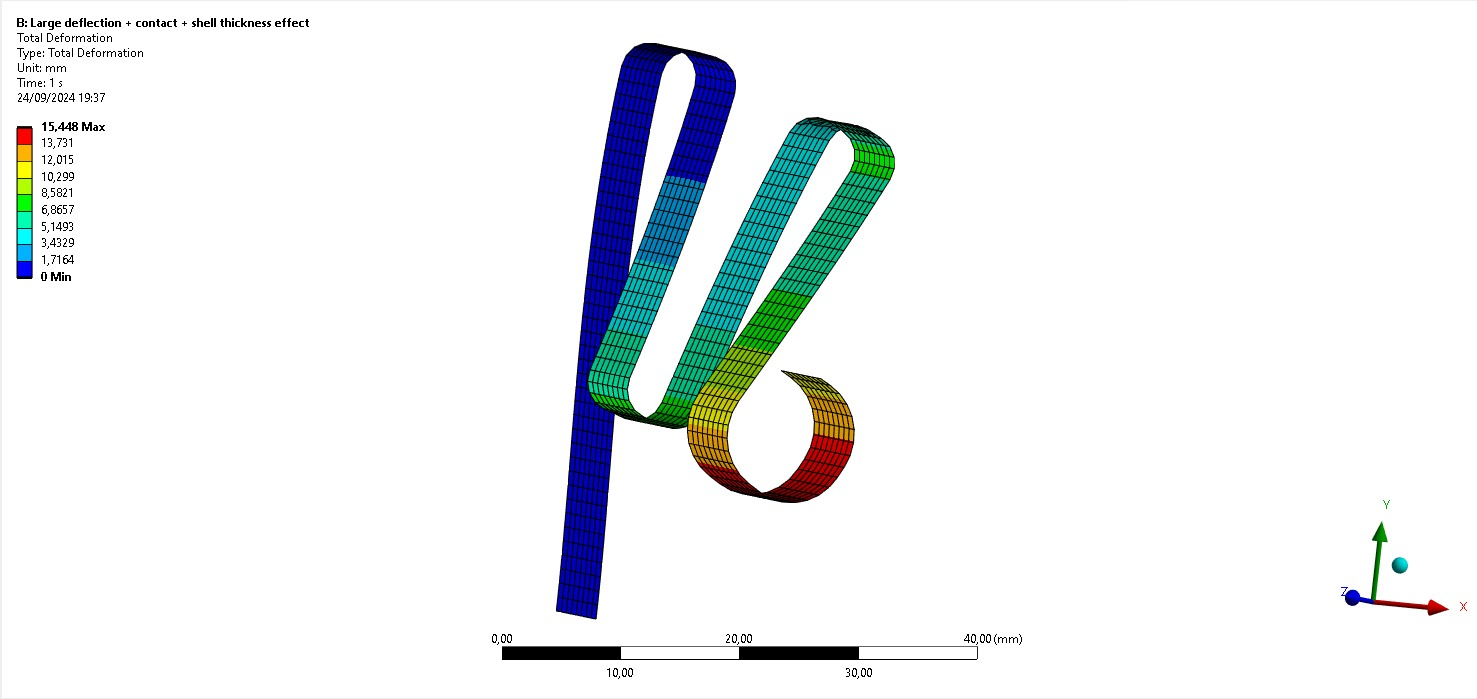
\includegraphics[width=0.7\linewidth]{Imagens/deformação total nao linear.jpeg}
    \smallcaption{Fonte: Autor}
    \label{fig: defnl}
\end{figure}

A Figura \ref{fig: convergencia} mostra o gráfico de convergência da força em comportamento linear.


\begin{figure}[!htb]
    \centering
    \caption{Gráfico de convergência de força}
    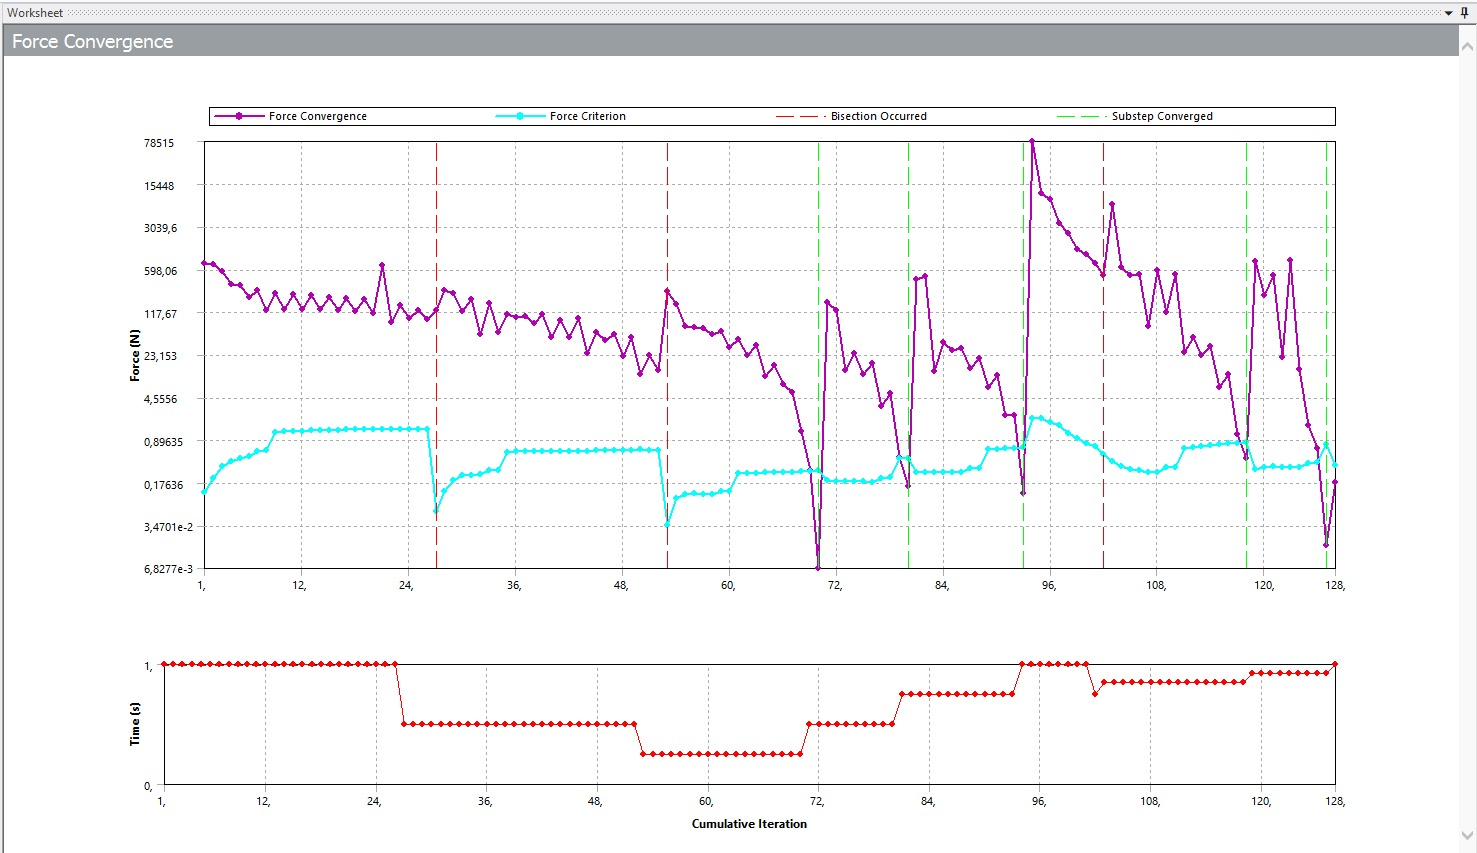
\includegraphics[width=0.7\linewidth]{Imagens/convergencia da força nao linear.jpeg}
    \smallcaption{Fonte: Autor}
    \label{fig: convergencia}
\end{figure}

\chapter{Conclusões}

Pode-se concluir que para a análise feita as não linearidades foram bem mais benéficas para a geometria, pois diminuiu sua deformação total e também a tensão equivalente. E como já dito antes, seria ideal trocar o material da mola para um material ideal para o objeto. 

Vale ressaltar, que o tipo de contato, a força aplicada e a espessura da geometria também interferem no resultado final.



\printbibliography

\end{document}

